\newpage
\section{Details and ablations for section~\ref{sec:calibrating_models}}
\label{sec:calibrating_models_appendix_experiments}

We begin by giving more experimental details. Note that the code is available in the supplementary folder for completeness.

We detail our experimental protocol for CIFAR-10 first. The CIFAR-10 validation set has 10,000 data points. We sampled, with replacement, a recalibration set of 1,000 points. In our theoretical approach and analysis, we split up these sets into multiple parts. For example, we used the first part for training a function, second part for bin construction, third part for binning. In practice, using the same set for all three steps worked out better, for both histogram binning and our variance-reduced binning approach. We believe that there may be theoretical justification for merging these sets, although we leave that for future work. For the marginal calibration experiment we ran either the variance-reduced calibrator (we fit a sigmoid in the function fitting step) or histogram binning. We calibrated each of the $K$ classes seprately as described in Section~\ref{sec:formulation}, and measured the marginal calibration error on the entire set of 10K points. We repeated this entire procedure 100 times, and computed mean and 90\% confidence intervals.

\begin{figure}
  \centering
  \centering
  	 \begin{subfigure}[b]{0.48\textwidth}
         \centering
         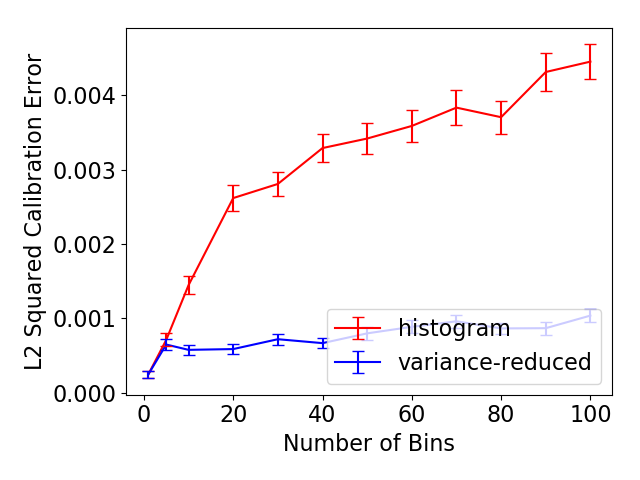
\includegraphics[width=\textwidth]{top_ces_imagenet.png}
         \caption{Effect of number of bins $B$ on top calibration error $\topsquaredce$ on ImageNet.
         }
         \label{fig:imagenet_top_cal_var_red}
     \end{subfigure}
     \hfill
     \begin{subfigure}[b]{0.48\textwidth}
         \centering
         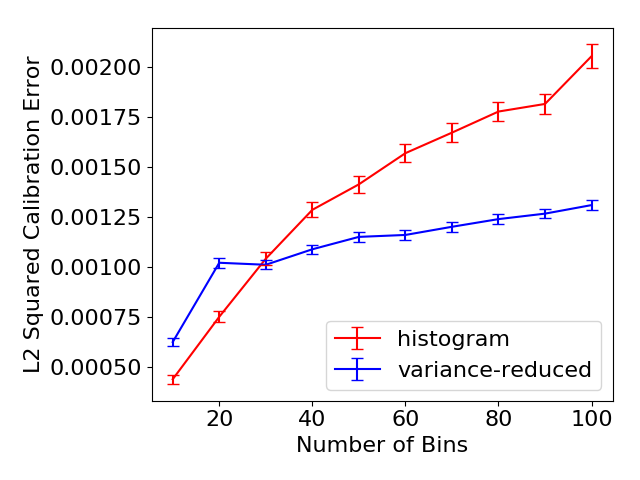
\includegraphics[width=\textwidth]{top_ces_cifar_1000.png}
         \caption{Effect of number of bins $B$ on top calibration error $\topsquaredce$ on CIFAR-10.
         }
         \label{fig:cifar_top_cal_var_red}
     \end{subfigure}
  \caption{
    Recalibrating using 1,000 data points on ImageNet and CIFAR-10, our variance-reduced calibrator typically achieves lower $\ell_2^2$ calibration error than histogram binning, especially when the number of bins $B$ is large. The difference is very significant on ImageNet, where our method does better when $B \geq 10$, and gets a nearly 5 times lower calibration error when $B = 100$. For CIFAR-10 our method does better when $B > 30$, which supports the theory which predicts that our method does better when $B$ is large. However, when $B$ is small, practitioners should try both histogram binning and the variance-reduced calibrator.
}
  \label{fig:mse_estimators_bins}
\end{figure}

In this experiment, we are checking a very precise hypothesis---assuming that the empirical distribution on the 10,000 validation points is the true data distribution, how do these methods perform? This is similar to the experimental protocol used in e.g.~\cite{brocker2012empirical}.
% This is not the same as an alternative hypothesis---how do these methods perform on the true CIFAR-10 distribution, which we do not have access to.
An alternative experimental protocol would have been to first split the CIFAR-10 data into two sets of size $(1000, 9000)$.
We could have then used the first set to recalibrate the model using either the variance-reduced calibrator or histogram binning, and then used the remaining 9,000 examples to estimate the calibration error on the ground truth distribution, using Bootstrap to compute confidence intervals.
However, when we ran this experiment, we noticed that the results were very sensitive to which set of 1,000 points we used to recalibrate.
Multiple runs of this experiment led to very different results.
The point is that there are two sources of randomness---the randomness in the data the recalibration method operates on, and the randomness in the data used to evaluate and compare the recalibrators.
In our protocol we account for both of these sources of randomness.

We also ran experiments on top-label calibration, for both ImageNet and CIFAR-10. The protocol is exactly as described above, except instead of calibrating each of the $K$ classes, we calibrated the top probability prediction of the model. More concretely, for each input $x_i$, the uncalibrated model outputs a probability $p_i$ corresponding to its top prediction $k_i$, where the true label is $y_i$. We create a new dataset $\{(p_1, \mathbb{I}(k_1 = y_1)), \dots, (p_n, \mathbb{I}(k_n = y_n))\}$ and run our variance-reduced calibration method (fitting a sigmoid in the function fitting step, as in Platt scaling) or histogram binning on this dataset, using $B$ bins. This calibrates the probability corresponding to the top prediction of the model. We evaluate the recalibrated models on the top-label calibration error metric ($\topsquaredce{}$) described in Section~\ref{sec:formulation}. For both CIFAR-10 and ImageNet we sampled, with replacement, a recalibration set of 1,000 points for the recalibration data, and we measured the calibration error on the entire set (10,000 points for CIFAR-10, and 50,000 points for ImageNet) as above. We show $90\%$ confidence intervals for all plots.

Figure~\ref{fig:imagenet_top_cal_var_red} shows that on ImageNet the variance-reduced calibrator gets significantly lower calibration errors than histogram binning when $B \geq 10$, and nearly a 5 times lower calibration error when $B = 100$. Both methods get similar calibration errors when $B = 1$ or $B = 5$. Figure~\ref{fig:cifar_top_cal_var_red} shows that on CIFAR-10 when $B$ is high, the variance-reduced calibrator gets lower calibration errors than histogram binning, but when $B$ is low histogram binning gets lower calibration errors. We believe that the difference might be because the CIFAR-10 model is highly accurate at top-label prediction to begin with, getting an accuracy of over $93\%$, so there is not much scope for re-calibration. In any case, this ablation tells us that practitioners should try multiple methods when recalibrating their models and evaluate their calibration error.
